\documentclass[]{thesis-ekf}
\usepackage[T1]{fontenc}
\PassOptionsToPackage{defaults=hu-min}{magyar.ldf}
\usepackage[magyar]{babel}
\usepackage{mathtools,amssymb,amsthm,pdfpages}
\footnotestyle{rule=fourth}

\newtheorem{tetel}{Tétel}[chapter]
\theoremstyle{definition}
\newtheorem{definicio}[tetel]{Definíció}
\theoremstyle{remark}
\newtheorem{megjegyzes}[tetel]{Megjegyzés}

\begin{document}

\institute{Matematikai és Informatikai Intézet}
\title{Szkenner megvalósítása egér szenzorral}
\author{Bodnár Máté\\Programtervező informatikus BSc}
\supervisor{Dr. Geda Gábor\\Egyetemi docens}
\city{Eger}
\date{2024}
\maketitle

\tableofcontents

\chapter*{Bevezetés}
\addcontentsline{toc}{chapter}{Bevezetés}
A digitalizálás egyre nagyobb szerepet játszik az életünkben, különösen a dokumentumok kezelésében és tárolásában, hiszen a sok ideig tárolt papír dokumentumok elveszhetnek vagy könnyen sérülhetnek.

Manapság a családi fotókat vagy régebbi képeket is célszerű digitalizálni, hogy tovább megmaradjon. A digitalizálással lehetőségünk nyílik arra is hogy rendszerezzünk hivatalos iratokat, így könnyebben tudunk majd hozzájuk férni és akár keresni is köztük. 

Bár számos szkenner van a piacon, viszont ezek drágák és nagy helyigényűek. Ezért egy saját készítésű szkenner jobban illeszkedik majd a mi igényeinkhez, valamint sokkal olcsóbb mint egy boltban vett. 

Ebben a projektben megmutatom hogy lehet egy egérszenzort felhasználni hivatalos iratok vagy egyéb más papír alapú dokumentumok szkennelésére. A szenzor két sínnel vízszintesen és függőlegesen fog mozogni, és soronként készíti el a képkockákat. Ezután egy C\# alkalmazás feldolgozza azokat és ki alakít belőlük egy nagy dokumentumot.

\chapter{Bevezető}

\section{Motiváció}
Az ötletem mögött több tényező is áll. Elsősorban szerettem volna egy olyan eszközt létrehozni, amely megfizethető alternatívát nyújt a drága szkennerekkel szemben. Az egérszenzorok könnyen beszerezhetők és viszonylag olcsók, ezért jó választásnak tűntek egy saját fejlesztésű szkennerhez. Ez különösen hasznos lehet olyan helyeken, ahol a költségek csökkentése nagyon fontos, például iskolákban vagy kisebb cégeknél.

Mindig is érdekelt, hogyan lehet egy meglévő egyszerű technológiát új és kreatív módon felhasználni. Az egérszenzorokat alapvetően mozgásérzékelésre tervezték, de ebben a projektben megszeretném mutatni, hogy dokumentumok szkennelésére is alkalmasak.

Emellett fontos számomra, hogy egy olyan eszközt alkossak, amelyet egy egyszerű felhasználó is használhat, otthon vagy akár a munkahelyén anélkül, hogy drága berendezésekre kellene költenie. 

Valamint kihívást látok ebben a projektben, hogy hogyan is tudom ezt megvalósítani. Izgalmas feladat az, hogy ötvözzem az informatikát az elektronikával. Ez nem csak a szakmai tudásomat fejleszti, hanem egy olyan eredményt ad, amelyre büszke lehetek.
\section{Célkitűzés}
A szakdolgozatom célja, egy olyan szkenner létrehozása, amely egy egyszerű egérszenzort használ a dokumentumok fekete-fehér beolvasására. Az eszköz működésének alapja, hogy a szenzor monokróm felvételeket készít a dokumentumról, majd ezeket egy számítógépes programmal feldolgozom és összeállítom egy nagy dokumentummá. Mivel a szenzor csak egy 30\,x\,30-as képet rögzít így azt interpolációval felnövelem. Ezek az algoritmusok lehetővé teszik, hogy a képet megnöveljük kevés minőség vesztéssel. 

A dolgozat eredményeként egy egyszerű és költséghatékony szkennert szeretnék létrehozni, amely hasznos és megkönnyíti az emberek életét.
\chapter{Felhaszánlt technológiák}
Ebben a fejezetben a szakdolgozatomban használt technológiákról és azok előnyeiről, fogok beszámolni.
\section{Arduino}
\subsection{Arduino platform bemutatása}
Az Arduino\cite{arduino} egy nyílt forráskódú platform amiket az elektronikai projektekhez találtak ki, majd bekerült az oktatásba is, oktatási céllal. Sokan használják egyszerűbb feladatok automatizálására vagy akár okos otthon rendszerek kialakítására. Ezek mellett manapság már az ipari alkalmazásuk sem ritka. A működéséhez szükség van egy mikrokontrollerre valamint egy fejlesztő környezetre az Arduino IDE-re, amivel általában USB kábelen keresztül tudjuk átküldeni a programot a fizikai eszközre.
\begin{figure}[th!]
	\centering
	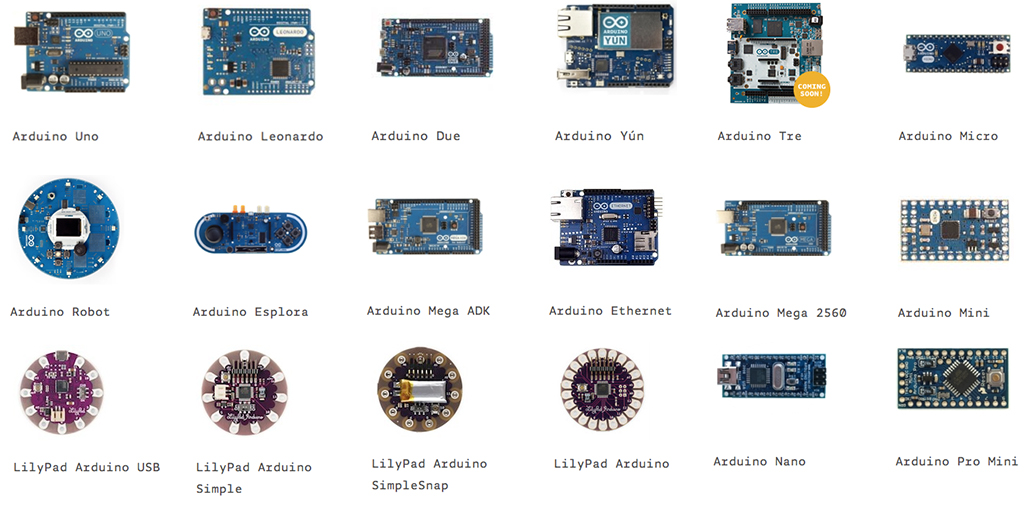
\includegraphics[width=0.9\linewidth]{ArduinoFamily}
	\caption[Arduino család néhány fajtája]{Arduino család néhány fajtája}
	\label{fig-arduinofamily}
\end{figure}
\subsection{Miért választottam az Arduino UNO-t?}
Szakdolgozatom során az Arduino UNO mellett dönöttem mivel több olyan előnye van ami fontos a projektem során.
\begin{itemize}
	\item \textbf{1. Egyszerű és széles körűen elterjedt és támogatott.} Széles körben elérhetőek könyvtárak és példakódok amik megkönnyítik a fejlesztést. Valamint ez a legjobban dokumentált mikrokontroller a felhasználók között.
	\item \textbf{2. Megfelelő teljesítmény és I/O portok.} Ez a mikrokontroller egy ATmega328P mikrovezérlőt használ mely megfelelő arra hogy kezeljem az egérszenzort és az RGB LED-et, valamint az adatok egyszerű továbbítására.
	\item \textbf{3. Megbízhatóság és stabilitás.} A stabilitás a projektem szempontjából nagyon fontos hisz hosszabb távon kell hiba mentes működést nyújtania, hiszen dokumentumok szkennelése közben folyamatos adatgyűjtésre és adatátvitelre van szükségem.
	\item \textbf{4. Költséghatékonyság.} Ez az egyik legolcsóbb fejlesztői eszköz, amely a kellő igényeket kielégíti a projektemhez.
	\item \textbf{5. Egyszerű programozhatóság valamint egyszerű kapcsolat.} Könnyen programozható mikrokontroller az Arduino IDE szoftverrel, és egyszerűen USB-n keresztül lehet áttölteni rá programokat.
\end{itemize}
\subsection{Arduino UNO}
Ez volt az egyik legelső és leginkább elterjedt mikrokontroller. Ezeknek az eszközöknek a szíve és lelke egy ATmega328P mikrovezérlő melyben található: 
\begin{itemize}
	\item Processzor
	\item Memória
	\item Különböző perifériák:
	\begin{itemize}
		\item Időzítő áramkörök
		\item Analóg és digitális be és kimenetek
		\item Kommunikációs perifériák és még sok egyéb
	\end{itemize}
\end{itemize}
\begin{figure}[th!]
	\centering
	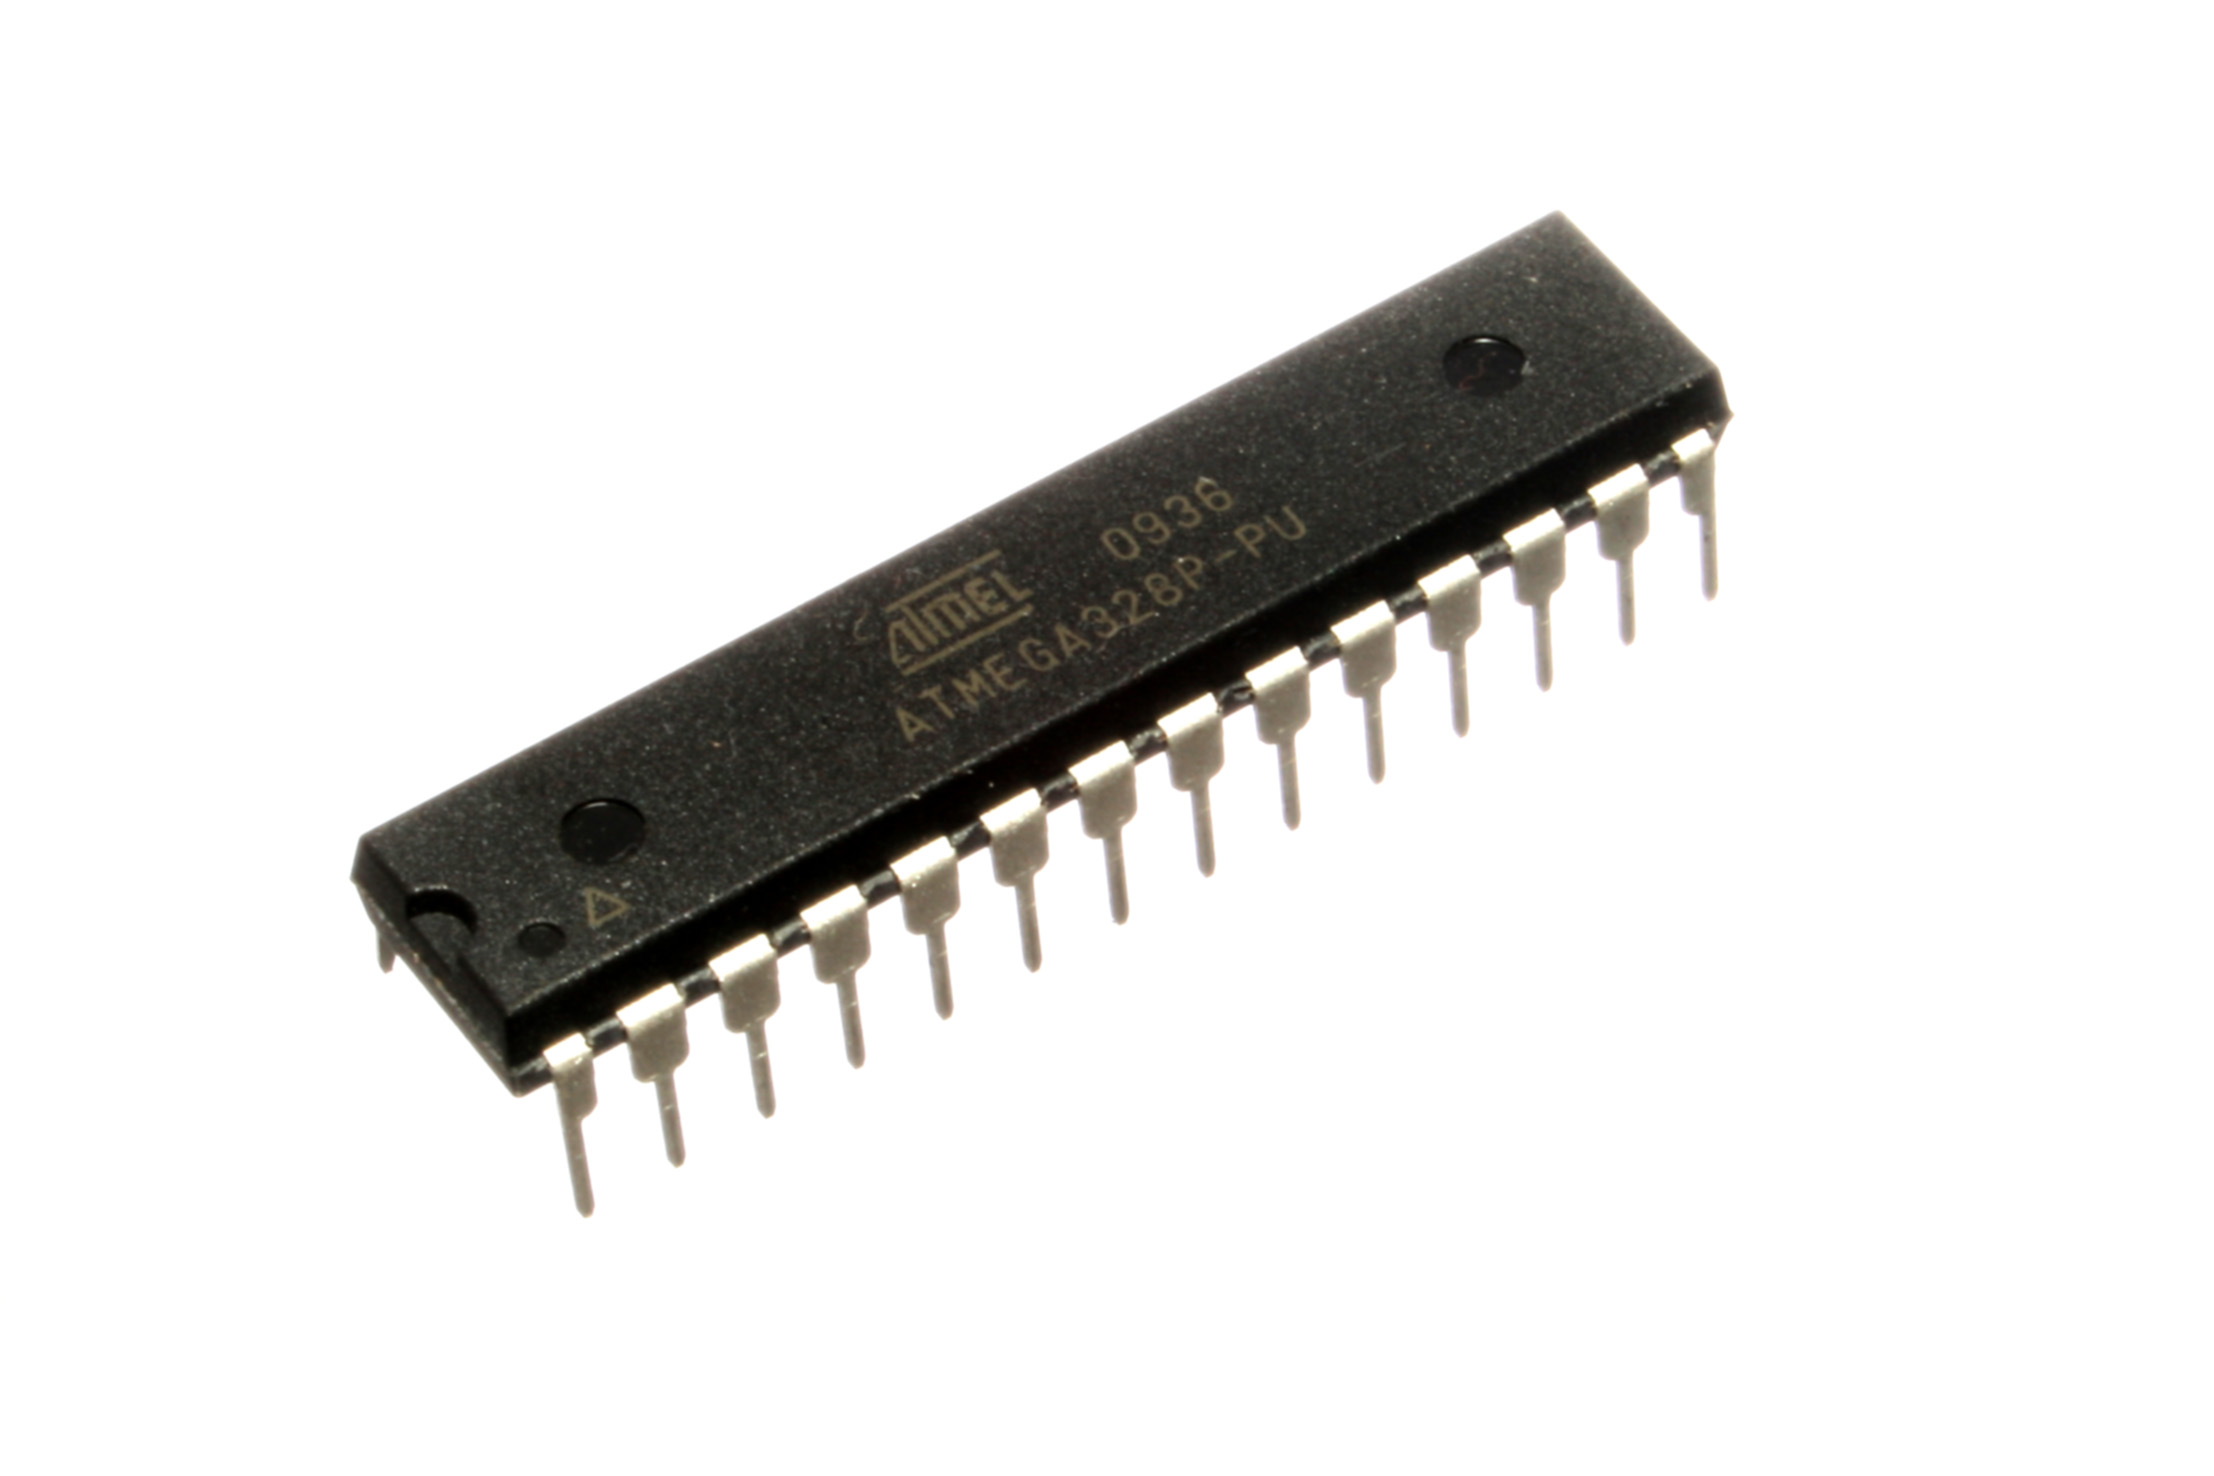
\includegraphics[width=0.4\linewidth]{ATMEGA328P-PU}
	\caption[ATmega328P]{ATmega328P mikrovezérlő}
	\label{fig:atmega328p-pu}
\end{figure}
\pagebreak
Ezek segítségével tudunk szenzorjeleket mérni, nyomógombok vagy más beviteli eszközök állapotát beolvasni. Az UNO áramkör szerepe hogy a mikrovezérlőnek a lábait kivezesse. Így kényelmesebben és egyszerűbben rá tudjuk kötni a különböző eszközöket amiket vezérelni szeretnénk, vagy értékeket beolvasni róluk. 

A mikrokontrollereken általában nem szokott futni operációs rendszer, ezért minden erőforrást a feladatra összpontosít és egy garantált maximális idő alatt képes végre hajtani a feladatokat. 

Ahhoz hogy külső eszközöket és áramköröket rátudjunk csatlakoztatni, ismernünk kell az UNO lábkiosztását, amikre a kódból tudunk hivatkozni és vezérelni őket. Az Arduino UNO áramköri lapon fel van tüntetve, hogy melyik lábat melyik számmal érjük el. A kimenetek lehetnek digitálisak 0--13-ig vagy analóg bemenetek A0--A5-ig. Az analóg bemenetek működhetnek digitális ki vagy bemenetekként, ez attól függ, hogy hogy állítjuk be a kódban. Van fix feszültséget leadó kivezetés is amelyen akár 3.3\,V-ot vagy 5\,V-ot is leadhatunk. Ezeket szemlélteti \aref{fig-arduinoparts}. számú ábra.
\begin{figure}[th!]
	\centering
	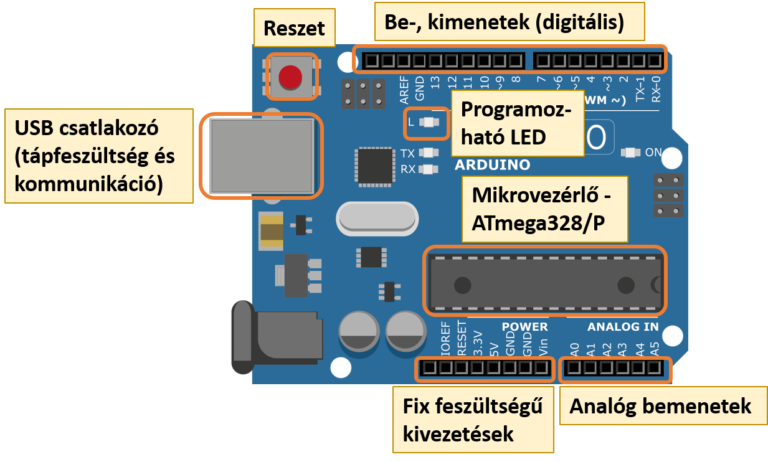
\includegraphics[width=0.7\linewidth]{ArduinoParts}
	\caption{Az Arduino UNO részei}
	\label{fig-arduinoparts}
\end{figure}
\subsection{Az Arduino alkalmazási területei}
\begin{itemize}
	\item \textbf{Kezdő projektekhez.} Az Arduino Board-ok tökéletesek a kezdők számára akik az elektronikát és az informatikát szeretnék ötvözni. A fejlesztő környezetet egyszerű kezelni valamint a könyvtárak és a példa kódok is nagyon sokat segítenek azoknak az embereknek akik elkezdenek érdeklődni az ilyen dolgok iránt.
	\item \textbf{Oktatási platform.} Könnyen kezelhetősége miatt szokták alkalmazni, hogy ezekkel az eszközökkel tanítsák meg az elektronika és az informatika működését.
	\item \textbf{Robotikában.} A nagy vállalatok vezetői is felfedezték ezt a technológiát, és gyakran Arduino Board-okat használnak a robotok megvalósításához és vezérléséhez.
	\item \textbf{Zene és művészet.} Az Arduino Board-okat szokták egyszerű hangszerek létrehozására is alkalmazni, vagy már meglévő hangszerekbe beépíteni elektronikus alkatrészként.
	\item \textbf{IoT - Internet of Things.} Legtöbb esetben okos otthon rendszerekbe szokták beépíteni, mert sok szenzort rá tudunk csatlakoztatni amikkel könnyen vezérelhetjük a saját otthonunkat. 
	\item \textbf{Viselhető eszközök. (Wearables)} Kompakt méretük miatt könnyen beépíthetőek ruhákba, akár ékszerekbe vagy más hordozható eszközökbe. Amelyekkel mozgásokra reagálhatunk mérhetünk testhőmérsékletet és még sok mást.
\end{itemize}
\section{Visual Studio}
A projekt szoftveres részét Visual Studio\cite{visual-studio} fejlesztői környezettel készítettem el, mert ez áll hozzám a legközelebb. Itt valósítottam meg az interpolációt a kép minőségvesztés nélküli növelését. Valamint a program irányító felületét is itt programoztam le. 
\section{Github}
A verziókövetéshez a Githubot\cite{github} használtam azon belül is a Github Desktop-ot, mellyel könnyen tudtam több platformon is dolgozni a projekten, valamint ha valamit elrontottam könnyen vissza tudtam állítani a projektet egy korábbi verzióra.
\chapter{Hardveres megvalósítás}
a szenzor mozgatását belevinni
\section{ADNS-9800 szenzor}
\subsection{Működése}
\subsection{Adatok beolvasása}
\section{Adatok továbbítása a Visual Studio felé}
arduino felől rs32 és a studio felé pedig serial
\section{Hardveres bekötés}
smartdraw, circuitikz
\chapter{Szoftveres megvalósítás}
kell mégegy az arduinohoz az arduino szenzor kezelés és szenzor mozgatás
egy alkalmazás amiről tudom kezelni a szkennelést
\section{Beolvasott értékek tárolása 3 dimenzós mátrixban}
adatszeerkezet amiben a beolvasott képet tároljuk
\section{Bikubik interpoláció}
\subsection{Működése}
Működésének alapjai, Matematikai leírása
\section{Mátrix átalakítása képpé}



\chapter*{Összegzés}
Tapasztalatok amiket szereztem a projekt megvalósítása közben
Tovabbfejlesztési gondolatok

színes vagy szürke képet szeretne beolvasni
soros porton küldok egy bitet hogy színes vagy szürke legyen a kép a studiobol
felbontásra vonatkozóan például  feles átfedéssel 
\addcontentsline{toc}{chapter}{Összegzés}
\chapter*{Források}
\ref{fig-arduinofamily}. ábra: \emph{https://predictabledesigns.com/wp-content/uploads/2017/10/HeroImage.png}
\begin{thebibliography}{2}
\addcontentsline{toc}{chapter}{\bibname}
\bibitem{arduino} Arduino: \emph{https://www.arduino.cc/en/Guide/Introduction}
\bibitem{visual-studio} Microsoft Visual Studio: \emph{https://visualstudio.microsoft.com/}
\bibitem{github} Github: \emph{https://github.com/}
\end{thebibliography}

% Aláírt, szkennelt nyilatkozat beillesztése a szakdolgozat végére
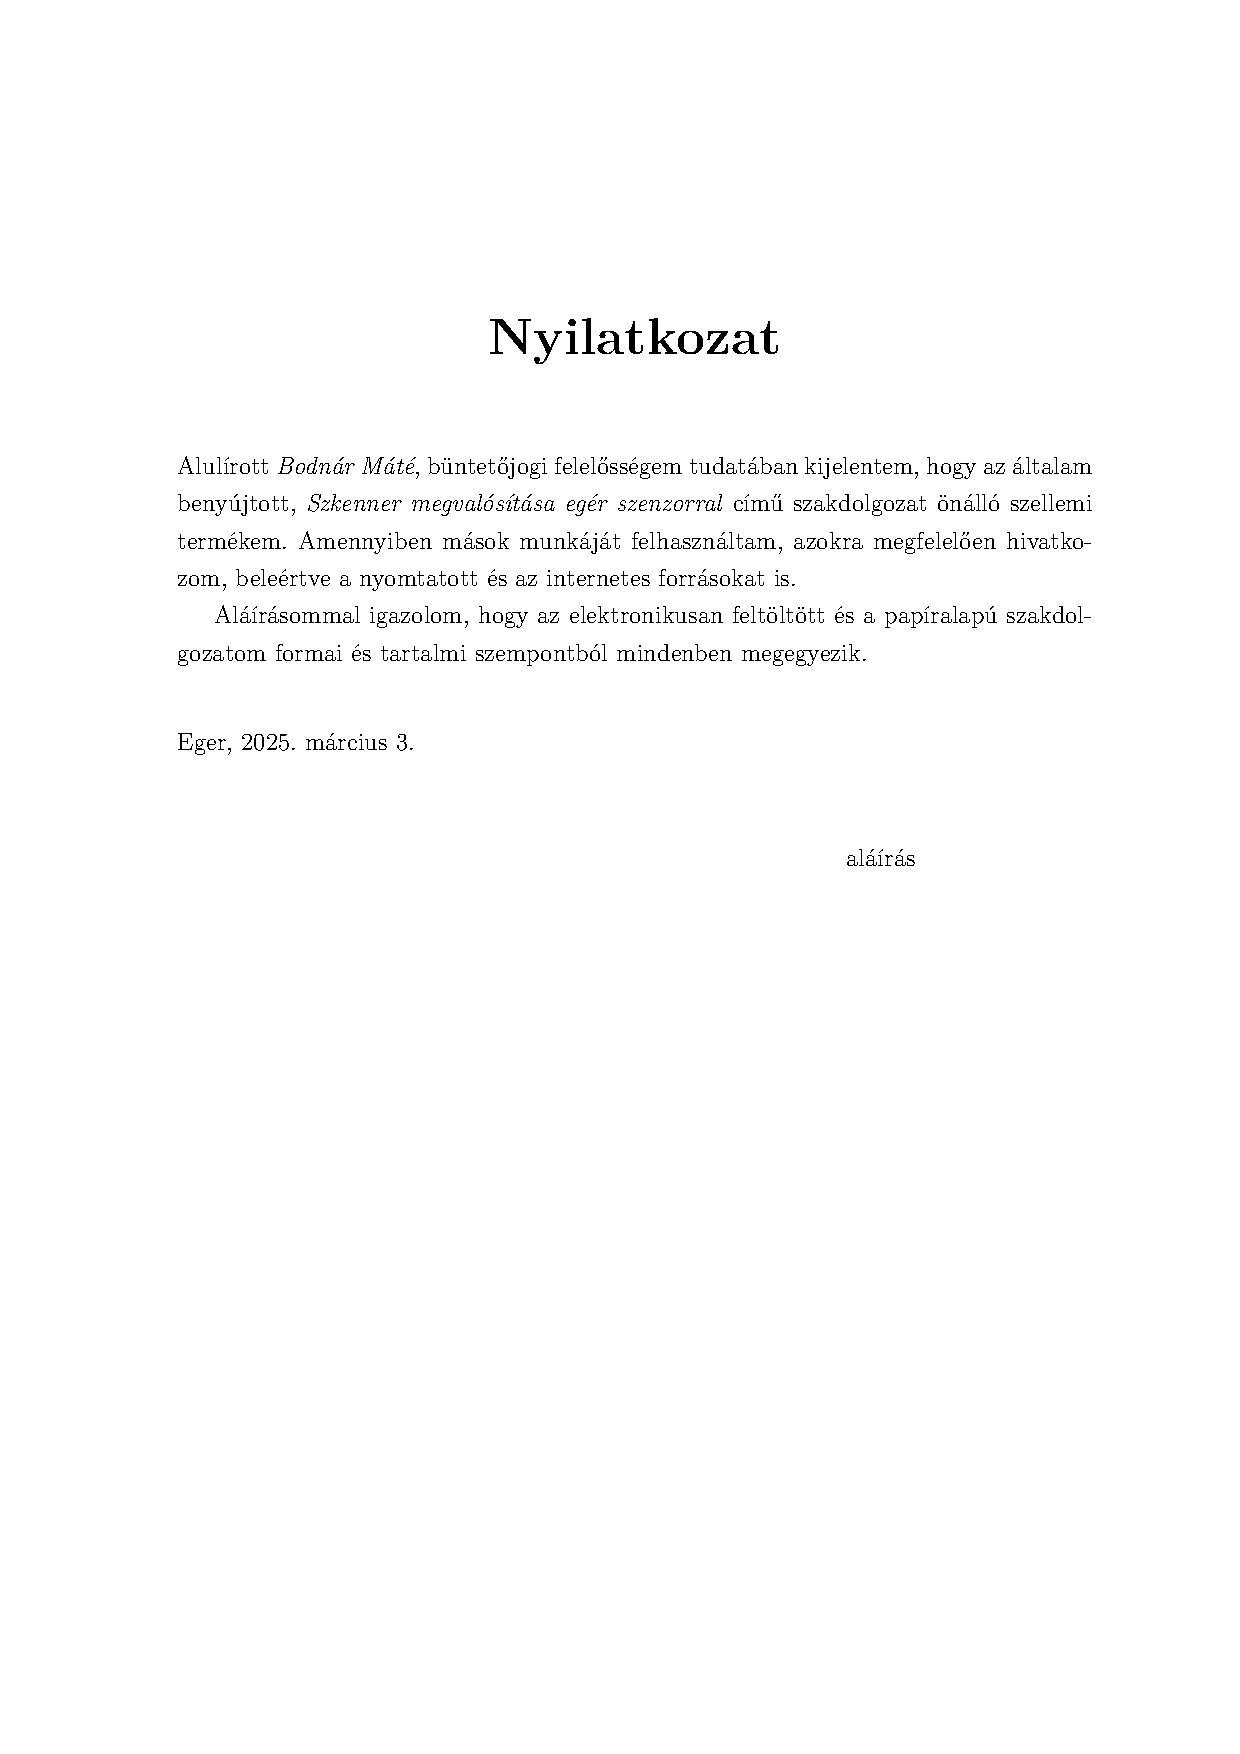
\includepdf{nyilatkozat.pdf}

\end{document}
